\documentclass[1p]{elsarticle_modified}
%\bibliographystyle{elsarticle-num}

%\usepackage[colorlinks]{hyperref}
%\usepackage{abbrmath_seonhwa} %\Abb, \Ascr, \Acal ,\Abf, \Afrak
\usepackage{amsfonts}
\usepackage{amssymb}
\usepackage{amsmath}
\usepackage{amsthm}
\usepackage{scalefnt}
\usepackage{amsbsy}
\usepackage{kotex}
\usepackage{caption}
\usepackage{subfig}
\usepackage{color}
\usepackage{graphicx}
\usepackage{xcolor} %% white, black, red, green, blue, cyan, magenta, yellow
\usepackage{float}
\usepackage{setspace}
\usepackage{hyperref}

\usepackage{tikz}
\usetikzlibrary{arrows}

\usepackage{multirow}
\usepackage{array} % fixed length table
\usepackage{hhline}

%%%%%%%%%%%%%%%%%%%%%
\makeatletter
\renewcommand*\env@matrix[1][\arraystretch]{%
	\edef\arraystretch{#1}%
	\hskip -\arraycolsep
	\let\@ifnextchar\new@ifnextchar
	\array{*\c@MaxMatrixCols c}}
\makeatother %https://tex.stackexchange.com/questions/14071/how-can-i-increase-the-line-spacing-in-a-matrix
%%%%%%%%%%%%%%%

\usepackage[normalem]{ulem}

\newcommand{\msout}[1]{\ifmmode\text{\sout{\ensuremath{#1}}}\else\sout{#1}\fi}
%SOURCE: \msout is \stkout macro in https://tex.stackexchange.com/questions/20609/strikeout-in-math-mode

\newcommand{\cancel}[1]{
	\ifmmode
	{\color{red}\msout{#1}}
	\else
	{\color{red}\sout{#1}}
	\fi
}

\newcommand{\add}[1]{
	{\color{blue}\uwave{#1}}
}

\newcommand{\replace}[2]{
	\ifmmode
	{\color{red}\msout{#1}}{\color{blue}\uwave{#2}}
	\else
	{\color{red}\sout{#1}}{\color{blue}\uwave{#2}}
	\fi
}

\newcommand{\Sol}{\mathcal{S}} %segment
\newcommand{\D}{D} %diagram
\newcommand{\A}{\mathcal{A}} %arc


%%%%%%%%%%%%%%%%%%%%%%%%%%%%%5 test

\def\sl{\operatorname{\textup{SL}}(2,\Cbb)}
\def\psl{\operatorname{\textup{PSL}}(2,\Cbb)}
\def\quan{\mkern 1mu \triangleright \mkern 1mu}

\theoremstyle{definition}
\newtheorem{thm}{Theorem}[section]
\newtheorem{prop}[thm]{Proposition}
\newtheorem{lem}[thm]{Lemma}
\newtheorem{ques}[thm]{Question}
\newtheorem{cor}[thm]{Corollary}
\newtheorem{defn}[thm]{Definition}
\newtheorem{exam}[thm]{Example}
\newtheorem{rmk}[thm]{Remark}
\newtheorem{alg}[thm]{Algorithm}

\newcommand{\I}{\sqrt{-1}}
\begin{document}

%\begin{frontmatter}
%
%\title{Boundary parabolic representations of knots up to 8 crossings}
%
%%% Group authors per affiliation:
%\author{Yunhi Cho} 
%\address{Department of Mathematics, University of Seoul, Seoul, Korea}
%\ead{yhcho@uos.ac.kr}
%
%
%\author{Seonhwa Kim} %\fnref{s_kim}}
%\address{Center for Geometry and Physics, Institute for Basic Science, Pohang, 37673, Korea}
%\ead{ryeona17@ibs.re.kr}
%
%\author{Hyuk Kim}
%\address{Department of Mathematical Sciences, Seoul National University, Seoul 08826, Korea}
%\ead{hyukkim@snu.ac.kr}
%
%\author{Seokbeom Yoon}
%\address{Department of Mathematical Sciences, Seoul National University, Seoul, 08826,  Korea}
%\ead{sbyoon15@snu.ac.kr}
%
%\begin{abstract}
%We find all boundary parabolic representation of knots up to 8 crossings.
%
%\end{abstract}
%\begin{keyword}
%    \MSC[2010] 57M25 
%\end{keyword}
%
%\end{frontmatter}

%\linenumbers
%\tableofcontents
%
\newcommand\colored[1]{\textcolor{white}{\rule[-0.35ex]{0.8em}{1.4ex}}\kern-0.8em\color{red} #1}%
%\newcommand\colored[1]{\textcolor{white}{ #1}\kern-2.17ex	\textcolor{white}{ #1}\kern-1.81ex	\textcolor{white}{ #1}\kern-2.15ex\color{red}#1	}

{\Large $\underline{12a_{0688}~(K12a_{0688})}$}

\setlength{\tabcolsep}{10pt}
\renewcommand{\arraystretch}{1.6}
\vspace{1cm}\begin{tabular}{m{100pt}>{\centering\arraybackslash}m{274pt}}
\multirow{5}{120pt}{
	\centering
	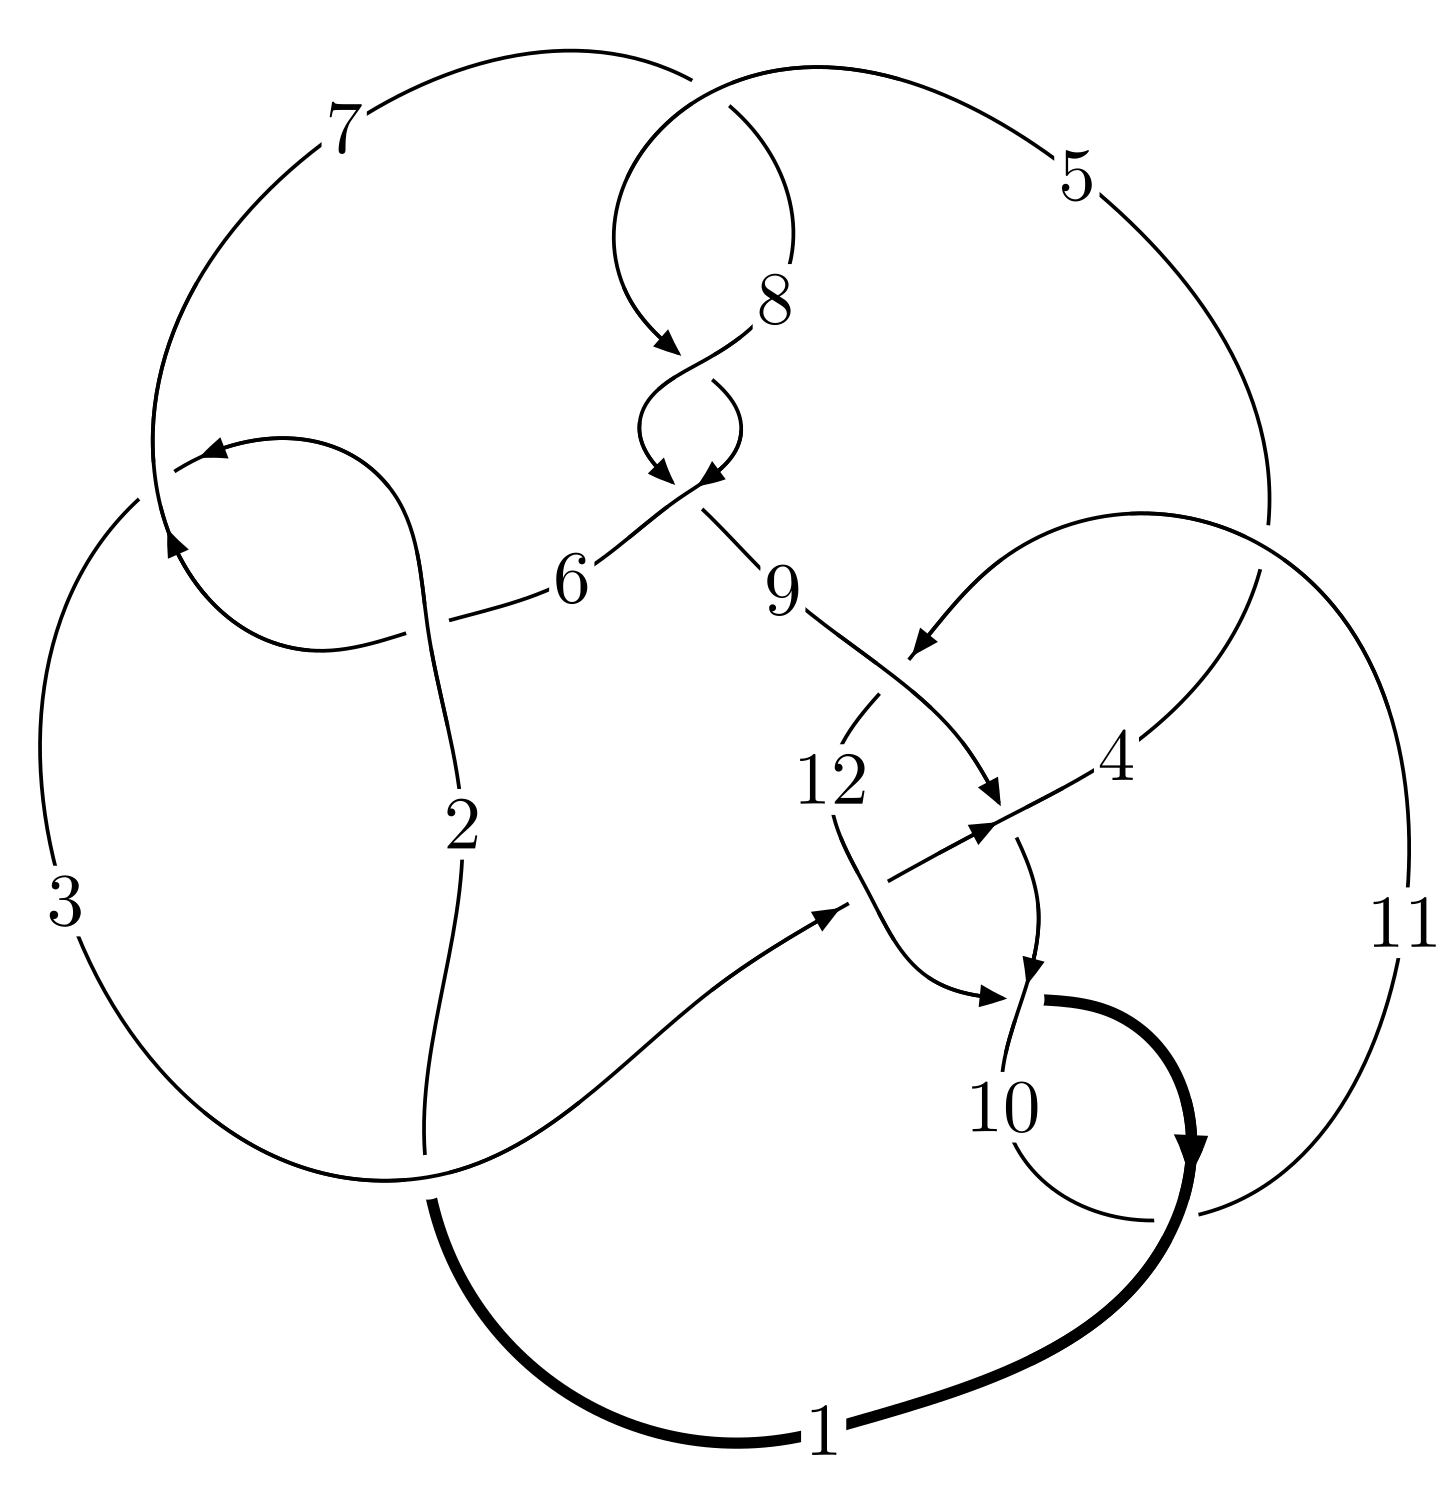
\includegraphics[width=112pt]{../../../GIT/diagram.site/Diagrams/png/1489_12a_0688.png}\\
\ \ \ A knot diagram\footnotemark}&
\allowdisplaybreaks
\textbf{Linearized knot diagam} \\
\cline{2-2}
 &
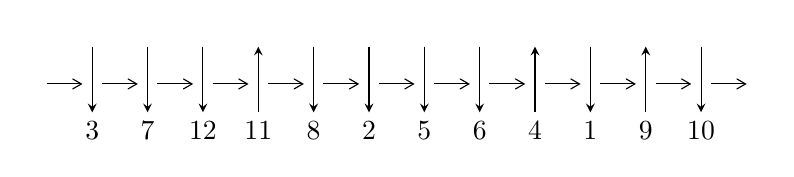
\begin{tikzpicture}[x=20pt, y=17pt]
	% nodes
	\node (C0) at (0, 0) {};
	\node (C1) at (1, 0) {};
	\node (C1U) at (1, +1) {};
	\node (C1D) at (1, -1) {3};

	\node (C2) at (2, 0) {};
	\node (C2U) at (2, +1) {};
	\node (C2D) at (2, -1) {7};

	\node (C3) at (3, 0) {};
	\node (C3U) at (3, +1) {};
	\node (C3D) at (3, -1) {12};

	\node (C4) at (4, 0) {};
	\node (C4U) at (4, +1) {};
	\node (C4D) at (4, -1) {11};

	\node (C5) at (5, 0) {};
	\node (C5U) at (5, +1) {};
	\node (C5D) at (5, -1) {8};

	\node (C6) at (6, 0) {};
	\node (C6U) at (6, +1) {};
	\node (C6D) at (6, -1) {2};

	\node (C7) at (7, 0) {};
	\node (C7U) at (7, +1) {};
	\node (C7D) at (7, -1) {5};

	\node (C8) at (8, 0) {};
	\node (C8U) at (8, +1) {};
	\node (C8D) at (8, -1) {6};

	\node (C9) at (9, 0) {};
	\node (C9U) at (9, +1) {};
	\node (C9D) at (9, -1) {4};

	\node (C10) at (10, 0) {};
	\node (C10U) at (10, +1) {};
	\node (C10D) at (10, -1) {1};

	\node (C11) at (11, 0) {};
	\node (C11U) at (11, +1) {};
	\node (C11D) at (11, -1) {9};

	\node (C12) at (12, 0) {};
	\node (C12U) at (12, +1) {};
	\node (C12D) at (12, -1) {10};
	\node (C13) at (13, 0) {};

	% arrows
	\draw[->,>={angle 60}]
	(C0) edge (C1) (C1) edge (C2) (C2) edge (C3) (C3) edge (C4) (C4) edge (C5) (C5) edge (C6) (C6) edge (C7) (C7) edge (C8) (C8) edge (C9) (C9) edge (C10) (C10) edge (C11) (C11) edge (C12) (C12) edge (C13) ;	\draw[->,>=stealth]
	(C1U) edge (C1D) (C2U) edge (C2D) (C3U) edge (C3D) (C4D) edge (C4U) (C5U) edge (C5D) (C6U) edge (C6D) (C7U) edge (C7D) (C8U) edge (C8D) (C9D) edge (C9U) (C10U) edge (C10D) (C11D) edge (C11U) (C12U) edge (C12D) ;
	\end{tikzpicture} \\
\hhline{~~} \\& 
\textbf{Solving Sequence} \\ \cline{2-2} 
 &
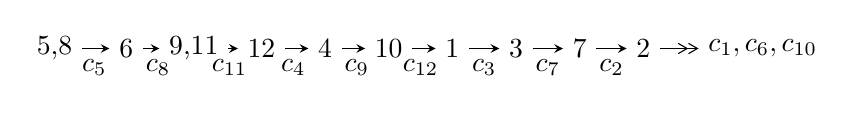
\begin{tikzpicture}[x=23pt, y=7pt]
	% node
	\node (A0) at (-1/8, 0) {5,8};
	\node (A1) at (1, 0) {6};
	\node (A2) at (33/16, 0) {9,11};
	\node (A3) at (25/8, 0) {12};
	\node (A4) at (33/8, 0) {4};
	\node (A5) at (41/8, 0) {10};
	\node (A6) at (49/8, 0) {1};
	\node (A7) at (57/8, 0) {3};
	\node (A8) at (65/8, 0) {7};
	\node (A9) at (73/8, 0) {2};
	\node (C1) at (1/2, -1) {$c_{5}$};
	\node (C2) at (3/2, -1) {$c_{8}$};
	\node (C3) at (21/8, -1) {$c_{11}$};
	\node (C4) at (29/8, -1) {$c_{4}$};
	\node (C5) at (37/8, -1) {$c_{9}$};
	\node (C6) at (45/8, -1) {$c_{12}$};
	\node (C7) at (53/8, -1) {$c_{3}$};
	\node (C8) at (61/8, -1) {$c_{7}$};
	\node (C9) at (69/8, -1) {$c_{2}$};
	\node (A10) at (11, 0) {$c_{1},c_{6},c_{10}$};

	% edge
	\draw[->,>=stealth]	
	(A0) edge (A1) (A1) edge (A2) (A2) edge (A3) (A3) edge (A4) (A4) edge (A5) (A5) edge (A6) (A6) edge (A7) (A7) edge (A8) (A8) edge (A9) ;
	\draw[->>,>={angle 60}]	
	(A9) edge (A10);
\end{tikzpicture} \\ 

\end{tabular} \\

\footnotetext{
The image of knot diagram is generated by the software ``\textbf{Draw programme}" developed by Andrew Bartholomew(\url{http://www.layer8.co.uk/maths/draw/index.htm\#Running-draw}), where we modified some parts for our purpose(\url{https://github.com/CATsTAILs/LinksPainter}).
}\phantom \\ \newline 
\centering \textbf{Ideals for irreducible components\footnotemark of $X_{\text{par}}$} 
 
\begin{align*}
I^u_{1}&=\langle 
1.68453\times10^{93} u^{111}+1.11304\times10^{94} u^{110}+\cdots+1.28372\times10^{91} b+1.22997\times10^{93},\\
\phantom{I^u_{1}}&\phantom{= \langle  }9.04813\times10^{92} u^{111}+6.05101\times10^{93} u^{110}+\cdots+6.41862\times10^{90} a+6.86529\times10^{92},\;u^{112}+8 u^{111}+\cdots+7 u+1\rangle \\
I^u_{2}&=\langle 
-3 a^5-13 a^4-7 a^3+17 a^2+13 b-21 a-7,\;a^6+6 a^5+11 a^4+4 a^3- a^2+a+1,\;u-1\rangle \\
I^u_{3}&=\langle 
b- u-2,\;a+2 u+3,\;u^2+u-1\rangle \\
\\
\end{align*}
\raggedright * 3 irreducible components of $\dim_{\mathbb{C}}=0$, with total 120 representations.\\
\footnotetext{All coefficients of polynomials are rational numbers. But the coefficients are sometimes approximated in decimal forms when there is not enough margin.}
\newpage
\renewcommand{\arraystretch}{1}
\centering \section*{I. $I^u_{1}= \langle 1.68\times10^{93} u^{111}+1.11\times10^{94} u^{110}+\cdots+1.28\times10^{91} b+1.23\times10^{93},\;9.05\times10^{92} u^{111}+6.05\times10^{93} u^{110}+\cdots+6.42\times10^{90} a+6.87\times10^{92},\;u^{112}+8 u^{111}+\cdots+7 u+1 \rangle$}
\flushleft \textbf{(i) Arc colorings}\\
\begin{tabular}{m{7pt} m{180pt} m{7pt} m{180pt} }
\flushright $a_{5}=$&$\begin{pmatrix}1\\0\end{pmatrix}$ \\
\flushright $a_{8}=$&$\begin{pmatrix}0\\u\end{pmatrix}$ \\
\flushright $a_{6}=$&$\begin{pmatrix}1\\u^2\end{pmatrix}$ \\
\flushright $a_{9}=$&$\begin{pmatrix}- u\\- u^3+u\end{pmatrix}$ \\
\flushright $a_{11}=$&$\begin{pmatrix}-140.967 u^{111}-942.728 u^{110}+\cdots-600.909 u-106.959\\-131.222 u^{111}-867.039 u^{110}+\cdots-599.242 u-95.8125\end{pmatrix}$ \\
\flushright $a_{12}=$&$\begin{pmatrix}-213.060 u^{111}-1409.07 u^{110}+\cdots-894.420 u-152.892\\-224.762 u^{111}-1481.90 u^{110}+\cdots-1006.45 u-160.281\end{pmatrix}$ \\
\flushright $a_{4}=$&$\begin{pmatrix}395.197 u^{111}+2586.54 u^{110}+\cdots+1658.16 u+259.193\\480.110 u^{111}+3139.69 u^{110}+\cdots+2114.70 u+332.176\end{pmatrix}$ \\
\flushright $a_{10}=$&$\begin{pmatrix}-222.614 u^{111}-1474.78 u^{110}+\cdots-971.574 u-159.791\\-210.094 u^{111}-1388.78 u^{110}+\cdots-955.661 u-152.161\end{pmatrix}$ \\
\flushright $a_{1}=$&$\begin{pmatrix}29.6253 u^{111}+191.679 u^{110}+\cdots+147.724 u+18.3331\\27.7910 u^{111}+186.215 u^{110}+\cdots+132.979 u+21.1686\end{pmatrix}$ \\
\flushright $a_{3}=$&$\begin{pmatrix}-11.9578 u^{111}-90.3909 u^{110}+\cdots-110.147 u-13.3668\\-1.04928 u^{111}-18.2756 u^{110}+\cdots-40.6199 u-7.10602\end{pmatrix}$ \\
\flushright $a_{7}=$&$\begin{pmatrix}u\\u\end{pmatrix}$ \\
\flushright $a_{2}=$&$\begin{pmatrix}8.04702 u^{111}+45.4206 u^{110}+\cdots-14.9838 u+1.78624\\18.9556 u^{111}+117.536 u^{110}+\cdots+54.5429 u+8.04702\end{pmatrix}$\\&\end{tabular}
\flushleft \textbf{(ii) Obstruction class $= -1$}\\~\\
\flushleft \textbf{(iii) Cusp Shapes $= 725.208 u^{111}+4779.01 u^{110}+\cdots+3630.85 u+563.580$}\\~\\
\newpage\renewcommand{\arraystretch}{1}
\flushleft \textbf{(iv) u-Polynomials at the component}\newline \\
\begin{tabular}{m{50pt}|m{274pt}}
Crossings & \hspace{64pt}u-Polynomials at each crossing \\
\hline $$\begin{aligned}c_{1}\end{aligned}$$&$\begin{aligned}
&u^{112}+42 u^{111}+\cdots+36864 u+4096
\end{aligned}$\\
\hline $$\begin{aligned}c_{2},c_{6}\end{aligned}$$&$\begin{aligned}
&u^{112}-2 u^{111}+\cdots+192 u+64
\end{aligned}$\\
\hline $$\begin{aligned}c_{3}\end{aligned}$$&$\begin{aligned}
&u^{112}-9 u^{111}+\cdots+2324 u-121
\end{aligned}$\\
\hline $$\begin{aligned}c_{4}\end{aligned}$$&$\begin{aligned}
&u^{112}-5 u^{111}+\cdots-32 u+161
\end{aligned}$\\
\hline $$\begin{aligned}c_{5},c_{7},c_{8}\end{aligned}$$&$\begin{aligned}
&u^{112}-8 u^{111}+\cdots-7 u+1
\end{aligned}$\\
\hline $$\begin{aligned}c_{9}\end{aligned}$$&$\begin{aligned}
&u^{112}+9 u^{111}+\cdots+2 u+1
\end{aligned}$\\
\hline $$\begin{aligned}c_{10},c_{12}\end{aligned}$$&$\begin{aligned}
&u^{112}-4 u^{111}+\cdots-35 u+1
\end{aligned}$\\
\hline $$\begin{aligned}c_{11}\end{aligned}$$&$\begin{aligned}
&u^{112}+18 u^{111}+\cdots-48 u+4
\end{aligned}$\\
\hline
\end{tabular}\\~\\
\newpage\renewcommand{\arraystretch}{1}
\flushleft \textbf{(v) Riley Polynomials at the component}\newline \\
\begin{tabular}{m{50pt}|m{274pt}}
Crossings & \hspace{64pt}Riley Polynomials at each crossing \\
\hline $$\begin{aligned}c_{1}\end{aligned}$$&$\begin{aligned}
&y^{112}+46 y^{111}+\cdots+1719664640 y+16777216
\end{aligned}$\\
\hline $$\begin{aligned}c_{2},c_{6}\end{aligned}$$&$\begin{aligned}
&y^{112}-42 y^{111}+\cdots-36864 y+4096
\end{aligned}$\\
\hline $$\begin{aligned}c_{3}\end{aligned}$$&$\begin{aligned}
&y^{112}-109 y^{111}+\cdots-1162588 y+14641
\end{aligned}$\\
\hline $$\begin{aligned}c_{4}\end{aligned}$$&$\begin{aligned}
&y^{112}-109 y^{111}+\cdots-254760 y+25921
\end{aligned}$\\
\hline $$\begin{aligned}c_{5},c_{7},c_{8}\end{aligned}$$&$\begin{aligned}
&y^{112}-96 y^{111}+\cdots+115 y+1
\end{aligned}$\\
\hline $$\begin{aligned}c_{9}\end{aligned}$$&$\begin{aligned}
&y^{112}+11 y^{111}+\cdots-8 y+1
\end{aligned}$\\
\hline $$\begin{aligned}c_{10},c_{12}\end{aligned}$$&$\begin{aligned}
&y^{112}-68 y^{111}+\cdots-815 y+1
\end{aligned}$\\
\hline $$\begin{aligned}c_{11}\end{aligned}$$&$\begin{aligned}
&y^{112}-18 y^{111}+\cdots-1464 y+16
\end{aligned}$\\
\hline
\end{tabular}\\~\\
\newpage\flushleft \textbf{(vi) Complex Volumes and Cusp Shapes}
$$\begin{array}{c|c|c}  
\text{Solutions to }I^u_{1}& \I (\text{vol} + \sqrt{-1}CS) & \text{Cusp shape}\\
 \hline 
\begin{aligned}
u &= \phantom{-}0.972143 + 0.332867 I \\
a &= -1.362640 - 0.348523 I \\
b &= \phantom{-}0.160167 + 0.470619 I\end{aligned}
 & -3.76699 + 1.68644 I & \phantom{-0.000000 } 0 \\ \hline\begin{aligned}
u &= \phantom{-}0.972143 - 0.332867 I \\
a &= -1.362640 + 0.348523 I \\
b &= \phantom{-}0.160167 - 0.470619 I\end{aligned}
 & -3.76699 - 1.68644 I & \phantom{-0.000000 } 0 \\ \hline\begin{aligned}
u &= \phantom{-}0.647072 + 0.675313 I \\
a &= \phantom{-}0.310613 + 0.510412 I \\
b &= -0.698002 + 0.997090 I\end{aligned}
 & -5.03852 - 7.34388 I & \phantom{-0.000000 } 0 \\ \hline\begin{aligned}
u &= \phantom{-}0.647072 - 0.675313 I \\
a &= \phantom{-}0.310613 - 0.510412 I \\
b &= -0.698002 - 0.997090 I\end{aligned}
 & -5.03852 + 7.34388 I & \phantom{-0.000000 } 0 \\ \hline\begin{aligned}
u &= \phantom{-}0.548793 + 0.737316 I \\
a &= -0.661657 + 0.301680 I \\
b &= -0.474652 - 0.832338 I\end{aligned}
 & -4.72741 + 2.38013 I & \phantom{-0.000000 } 0 \\ \hline\begin{aligned}
u &= \phantom{-}0.548793 - 0.737316 I \\
a &= -0.661657 - 0.301680 I \\
b &= -0.474652 + 0.832338 I\end{aligned}
 & -4.72741 - 2.38013 I & \phantom{-0.000000 } 0 \\ \hline\begin{aligned}
u &= \phantom{-}0.227920 + 0.890098 I \\
a &= -0.597510 - 0.463491 I \\
b &= \phantom{-}0.986400 - 0.352157 I\end{aligned}
 & \phantom{-}1.39228 - 6.23151 I & \phantom{-0.000000 } 0 \\ \hline\begin{aligned}
u &= \phantom{-}0.227920 - 0.890098 I \\
a &= -0.597510 + 0.463491 I \\
b &= \phantom{-}0.986400 + 0.352157 I\end{aligned}
 & \phantom{-}1.39228 + 6.23151 I & \phantom{-0.000000 } 0 \\ \hline\begin{aligned}
u &= \phantom{-}0.189834 + 0.893590 I \\
a &= \phantom{-}1.083890 + 0.384288 I \\
b &= -1.25320 + 1.19672 I\end{aligned}
 & \phantom{-}0.0844 - 14.1422 I & \phantom{-0.000000 } 0 \\ \hline\begin{aligned}
u &= \phantom{-}0.189834 - 0.893590 I \\
a &= \phantom{-}1.083890 - 0.384288 I \\
b &= -1.25320 - 1.19672 I\end{aligned}
 & \phantom{-}0.0844 + 14.1422 I & \phantom{-0.000000 } 0\\
 \hline 
 \end{array}$$\newpage$$\begin{array}{c|c|c}  
\text{Solutions to }I^u_{1}& \I (\text{vol} + \sqrt{-1}CS) & \text{Cusp shape}\\
 \hline 
\begin{aligned}
u &= \phantom{-}0.997496 + 0.551038 I \\
a &= \phantom{-}0.193992 - 0.279188 I \\
b &= \phantom{-}0.861494 + 0.198796 I\end{aligned}
 & -0.97322 + 1.18405 I & \phantom{-0.000000 } 0 \\ \hline\begin{aligned}
u &= \phantom{-}0.997496 - 0.551038 I \\
a &= \phantom{-}0.193992 + 0.279188 I \\
b &= \phantom{-}0.861494 - 0.198796 I\end{aligned}
 & -0.97322 - 1.18405 I & \phantom{-0.000000 } 0 \\ \hline\begin{aligned}
u &= \phantom{-}1.113020 + 0.261600 I \\
a &= -0.66056 + 3.72609 I \\
b &= -2.25960 - 0.15223 I\end{aligned}
 & -2.52074 - 0.67374 I & \phantom{-0.000000 } 0 \\ \hline\begin{aligned}
u &= \phantom{-}1.113020 - 0.261600 I \\
a &= -0.66056 - 3.72609 I \\
b &= -2.25960 + 0.15223 I\end{aligned}
 & -2.52074 + 0.67374 I & \phantom{-0.000000 } 0 \\ \hline\begin{aligned}
u &= \phantom{-}0.157978 + 0.840183 I \\
a &= -0.955571 - 0.661158 I \\
b &= \phantom{-}0.891203 - 0.911299 I\end{aligned}
 & \phantom{-}3.81295 - 7.90390 I & \phantom{-0.000000 } 0 \\ \hline\begin{aligned}
u &= \phantom{-}0.157978 - 0.840183 I \\
a &= -0.955571 + 0.661158 I \\
b &= \phantom{-}0.891203 + 0.911299 I\end{aligned}
 & \phantom{-}3.81295 + 7.90390 I & \phantom{-0.000000 } 0 \\ \hline\begin{aligned}
u &= \phantom{-}0.099726 + 0.831030 I \\
a &= \phantom{-}0.241531 + 0.125256 I \\
b &= -0.278553 + 0.649349 I\end{aligned}
 & \phantom{-}3.10964 - 3.02719 I & \phantom{-0.000000 } 0 \\ \hline\begin{aligned}
u &= \phantom{-}0.099726 - 0.831030 I \\
a &= \phantom{-}0.241531 - 0.125256 I \\
b &= -0.278553 - 0.649349 I\end{aligned}
 & \phantom{-}3.10964 + 3.02719 I & \phantom{-0.000000 } 0 \\ \hline\begin{aligned}
u &= \phantom{-}1.086720 + 0.423280 I \\
a &= \phantom{-}0.458631 + 0.411155 I \\
b &= \phantom{-}0.878136 + 0.769471 I\end{aligned}
 & \phantom{-}0.97833 + 3.36110 I & \phantom{-0.000000 } 0 \\ \hline\begin{aligned}
u &= \phantom{-}1.086720 - 0.423280 I \\
a &= \phantom{-}0.458631 - 0.411155 I \\
b &= \phantom{-}0.878136 - 0.769471 I\end{aligned}
 & \phantom{-}0.97833 - 3.36110 I & \phantom{-0.000000 } 0\\
 \hline 
 \end{array}$$\newpage$$\begin{array}{c|c|c}  
\text{Solutions to }I^u_{1}& \I (\text{vol} + \sqrt{-1}CS) & \text{Cusp shape}\\
 \hline 
\begin{aligned}
u &= -1.161640 + 0.221560 I \\
a &= \phantom{-}0.693593 - 0.043378 I \\
b &= \phantom{-}1.31955 - 0.74333 I\end{aligned}
 & -1.46335 - 4.79145 I & \phantom{-0.000000 } 0 \\ \hline\begin{aligned}
u &= -1.161640 - 0.221560 I \\
a &= \phantom{-}0.693593 + 0.043378 I \\
b &= \phantom{-}1.31955 + 0.74333 I\end{aligned}
 & -1.46335 + 4.79145 I & \phantom{-0.000000 } 0 \\ \hline\begin{aligned}
u &= -0.019986 + 0.809418 I \\
a &= -0.259392 + 0.443642 I \\
b &= \phantom{-}0.492698 + 0.239422 I\end{aligned}
 & \phantom{-}3.50998 - 2.86593 I & \phantom{-0.000000 } 0 \\ \hline\begin{aligned}
u &= -0.019986 - 0.809418 I \\
a &= -0.259392 - 0.443642 I \\
b &= \phantom{-}0.492698 - 0.239422 I\end{aligned}
 & \phantom{-}3.50998 + 2.86593 I & \phantom{-0.000000 } 0 \\ \hline\begin{aligned}
u &= \phantom{-}1.075340 + 0.518822 I \\
a &= -0.726902 + 0.037922 I \\
b &= -1.14674 - 1.11271 I\end{aligned}
 & -2.61261 + 9.14928 I & \phantom{-0.000000 } 0 \\ \hline\begin{aligned}
u &= \phantom{-}1.075340 - 0.518822 I \\
a &= -0.726902 - 0.037922 I \\
b &= -1.14674 + 1.11271 I\end{aligned}
 & -2.61261 - 9.14928 I & \phantom{-0.000000 } 0 \\ \hline\begin{aligned}
u &= \phantom{-}0.186766 + 0.778487 I \\
a &= -1.61668 + 0.23169 I \\
b &= \phantom{-}0.429062 - 0.334358 I\end{aligned}
 & -1.33438 - 5.79082 I & \phantom{-0.000000 } 0 \\ \hline\begin{aligned}
u &= \phantom{-}0.186766 - 0.778487 I \\
a &= -1.61668 - 0.23169 I \\
b &= \phantom{-}0.429062 + 0.334358 I\end{aligned}
 & -1.33438 + 5.79082 I & \phantom{-0.000000 } 0 \\ \hline\begin{aligned}
u &= \phantom{-}0.719187 + 0.318145 I \\
a &= -2.22822 - 0.73581 I \\
b &= \phantom{-}0.088142 - 0.899059 I\end{aligned}
 & -4.28499 - 1.36074 I & \phantom{-0.000000 } 0 \\ \hline\begin{aligned}
u &= \phantom{-}0.719187 - 0.318145 I \\
a &= -2.22822 + 0.73581 I \\
b &= \phantom{-}0.088142 + 0.899059 I\end{aligned}
 & -4.28499 + 1.36074 I & \phantom{-0.000000 } 0\\
 \hline 
 \end{array}$$\newpage$$\begin{array}{c|c|c}  
\text{Solutions to }I^u_{1}& \I (\text{vol} + \sqrt{-1}CS) & \text{Cusp shape}\\
 \hline 
\begin{aligned}
u &= \phantom{-}1.227110 + 0.002061 I \\
a &= -1.66017 + 1.94116 I \\
b &= -0.560265 + 0.316560 I\end{aligned}
 & -2.72849 - 1.53038 I & \phantom{-0.000000 } 0 \\ \hline\begin{aligned}
u &= \phantom{-}1.227110 - 0.002061 I \\
a &= -1.66017 - 1.94116 I \\
b &= -0.560265 - 0.316560 I\end{aligned}
 & -2.72849 + 1.53038 I & \phantom{-0.000000 } 0 \\ \hline\begin{aligned}
u &= -1.214510 + 0.193657 I \\
a &= -0.331320 - 0.319809 I \\
b &= -1.255610 - 0.094001 I\end{aligned}
 & -0.04609 + 2.27832 I & \phantom{-0.000000 } 0 \\ \hline\begin{aligned}
u &= -1.214510 - 0.193657 I \\
a &= -0.331320 + 0.319809 I \\
b &= -1.255610 + 0.094001 I\end{aligned}
 & -0.04609 - 2.27832 I & \phantom{-0.000000 } 0 \\ \hline\begin{aligned}
u &= \phantom{-}0.142386 + 0.756030 I \\
a &= \phantom{-}2.22149 + 0.27721 I \\
b &= -2.86360 - 0.28993 I\end{aligned}
 & \phantom{-}0.35372 - 3.11615 I & \phantom{-0.000000 } 0 \\ \hline\begin{aligned}
u &= \phantom{-}0.142386 - 0.756030 I \\
a &= \phantom{-}2.22149 - 0.27721 I \\
b &= -2.86360 + 0.28993 I\end{aligned}
 & \phantom{-}0.35372 + 3.11615 I & \phantom{-0.000000 } 0 \\ \hline\begin{aligned}
u &= \phantom{-}1.217360 + 0.250346 I \\
a &= \phantom{-}1.70418 - 3.04656 I \\
b &= \phantom{-}2.85131 + 0.00560 I\end{aligned}
 & -2.76825 - 1.54043 I & \phantom{-0.000000 } 0 \\ \hline\begin{aligned}
u &= \phantom{-}1.217360 - 0.250346 I \\
a &= \phantom{-}1.70418 + 3.04656 I \\
b &= \phantom{-}2.85131 - 0.00560 I\end{aligned}
 & -2.76825 + 1.54043 I & \phantom{-0.000000 } 0 \\ \hline\begin{aligned}
u &= \phantom{-}1.239890 + 0.163213 I \\
a &= -0.51282 - 2.72556 I \\
b &= -0.113281 - 1.084940 I\end{aligned}
 & -5.29466 - 0.57195 I & \phantom{-0.000000 } 0 \\ \hline\begin{aligned}
u &= \phantom{-}1.239890 - 0.163213 I \\
a &= -0.51282 + 2.72556 I \\
b &= -0.113281 + 1.084940 I\end{aligned}
 & -5.29466 + 0.57195 I & \phantom{-0.000000 } 0\\
 \hline 
 \end{array}$$\newpage$$\begin{array}{c|c|c}  
\text{Solutions to }I^u_{1}& \I (\text{vol} + \sqrt{-1}CS) & \text{Cusp shape}\\
 \hline 
\begin{aligned}
u &= -0.143570 + 0.726883 I \\
a &= -1.27103 + 0.68455 I \\
b &= \phantom{-}1.22226 + 1.00947 I\end{aligned}
 & \phantom{-}1.47470 + 8.28591 I & \phantom{-0.000000 } 0 \\ \hline\begin{aligned}
u &= -0.143570 - 0.726883 I \\
a &= -1.27103 - 0.68455 I \\
b &= \phantom{-}1.22226 - 1.00947 I\end{aligned}
 & \phantom{-}1.47470 - 8.28591 I & \phantom{-0.000000 } 0 \\ \hline\begin{aligned}
u &= -1.225750 + 0.333086 I \\
a &= \phantom{-}0.461927 - 0.047089 I \\
b &= \phantom{-}0.855537 - 0.095153 I\end{aligned}
 & -0.18525 + 6.98643 I & \phantom{-0.000000 } 0 \\ \hline\begin{aligned}
u &= -1.225750 - 0.333086 I \\
a &= \phantom{-}0.461927 + 0.047089 I \\
b &= \phantom{-}0.855537 + 0.095153 I\end{aligned}
 & -0.18525 - 6.98643 I & \phantom{-0.000000 } 0 \\ \hline\begin{aligned}
u &= -1.245720 + 0.276383 I \\
a &= -0.429395 + 0.363064 I \\
b &= -1.165230 + 0.702845 I\end{aligned}
 & \phantom{-}0.97470 + 1.25354 I & \phantom{-0.000000 } 0 \\ \hline\begin{aligned}
u &= -1.245720 - 0.276383 I \\
a &= -0.429395 - 0.363064 I \\
b &= -1.165230 - 0.702845 I\end{aligned}
 & \phantom{-}0.97470 - 1.25354 I & \phantom{-0.000000 } 0 \\ \hline\begin{aligned}
u &= -0.039317 + 0.720481 I \\
a &= \phantom{-}1.30484 - 0.79273 I \\
b &= -0.993124 - 0.771280 I\end{aligned}
 & \phantom{-}4.67418 + 2.34341 I & \phantom{-0.000000 } 0 \\ \hline\begin{aligned}
u &= -0.039317 - 0.720481 I \\
a &= \phantom{-}1.30484 + 0.79273 I \\
b &= -0.993124 + 0.771280 I\end{aligned}
 & \phantom{-}4.67418 - 2.34341 I & \phantom{-0.000000 } 0 \\ \hline\begin{aligned}
u &= \phantom{-}0.192939 + 0.694349 I \\
a &= -0.264401 + 0.563665 I \\
b &= \phantom{-}0.102997 + 1.191740 I\end{aligned}
 & -2.51350 - 2.16509 I & \phantom{-0.000000 } 0 \\ \hline\begin{aligned}
u &= \phantom{-}0.192939 - 0.694349 I \\
a &= -0.264401 - 0.563665 I \\
b &= \phantom{-}0.102997 - 1.191740 I\end{aligned}
 & -2.51350 + 2.16509 I & \phantom{-0.000000 } 0\\
 \hline 
 \end{array}$$\newpage$$\begin{array}{c|c|c}  
\text{Solutions to }I^u_{1}& \I (\text{vol} + \sqrt{-1}CS) & \text{Cusp shape}\\
 \hline 
\begin{aligned}
u &= \phantom{-}1.232290 + 0.347470 I \\
a &= -0.490318 - 0.822966 I \\
b &= \phantom{-}0.110576 - 0.543663 I\end{aligned}
 & -0.359065 - 1.357260 I & \phantom{-0.000000 } 0 \\ \hline\begin{aligned}
u &= \phantom{-}1.232290 - 0.347470 I \\
a &= -0.490318 + 0.822966 I \\
b &= \phantom{-}0.110576 + 0.543663 I\end{aligned}
 & -0.359065 + 1.357260 I & \phantom{-0.000000 } 0 \\ \hline\begin{aligned}
u &= \phantom{-}1.211410 + 0.426352 I \\
a &= -0.258603 - 0.333714 I \\
b &= -0.201500 - 0.178702 I\end{aligned}
 & -0.28499 - 1.43055 I & \phantom{-0.000000 } 0 \\ \hline\begin{aligned}
u &= \phantom{-}1.211410 - 0.426352 I \\
a &= -0.258603 + 0.333714 I \\
b &= -0.201500 + 0.178702 I\end{aligned}
 & -0.28499 + 1.43055 I & \phantom{-0.000000 } 0 \\ \hline\begin{aligned}
u &= \phantom{-}0.089830 + 0.703854 I \\
a &= -2.00704 - 0.17497 I \\
b &= \phantom{-}2.26623 - 0.37498 I\end{aligned}
 & \phantom{-}0.63350 - 1.90492 I & \phantom{-0.000000 } 0 \\ \hline\begin{aligned}
u &= \phantom{-}0.089830 - 0.703854 I \\
a &= -2.00704 + 0.17497 I \\
b &= \phantom{-}2.26623 + 0.37498 I\end{aligned}
 & \phantom{-}0.63350 + 1.90492 I & \phantom{-0.000000 } 0 \\ \hline\begin{aligned}
u &= \phantom{-}1.271470 + 0.237024 I \\
a &= \phantom{-}1.57652 + 0.70957 I \\
b &= -0.349469 + 0.426717 I\end{aligned}
 & -4.39307 - 4.01879 I & \phantom{-0.000000 } 0 \\ \hline\begin{aligned}
u &= \phantom{-}1.271470 - 0.237024 I \\
a &= \phantom{-}1.57652 - 0.70957 I \\
b &= -0.349469 - 0.426717 I\end{aligned}
 & -4.39307 + 4.01879 I & \phantom{-0.000000 } 0 \\ \hline\begin{aligned}
u &= \phantom{-}0.690432\phantom{ +0.000000I} \\
a &= -0.298400\phantom{ +0.000000I} \\
b &= \phantom{-}0.429439\phantom{ +0.000000I}\end{aligned}
 & -1.01489\phantom{ +0.000000I} & \phantom{-0.000000 } 0 \\ \hline\begin{aligned}
u &= \phantom{-}0.502927 + 0.470467 I \\
a &= -0.219491 - 1.265850 I \\
b &= \phantom{-}0.584208 - 0.484004 I\end{aligned}
 & -0.94679 - 3.25376 I & \phantom{-0.000000 } 0\\
 \hline 
 \end{array}$$\newpage$$\begin{array}{c|c|c}  
\text{Solutions to }I^u_{1}& \I (\text{vol} + \sqrt{-1}CS) & \text{Cusp shape}\\
 \hline 
\begin{aligned}
u &= \phantom{-}0.502927 - 0.470467 I \\
a &= -0.219491 + 1.265850 I \\
b &= \phantom{-}0.584208 + 0.484004 I\end{aligned}
 & -0.94679 + 3.25376 I & \phantom{-0.000000 } 0 \\ \hline\begin{aligned}
u &= \phantom{-}1.293630 + 0.299459 I \\
a &= \phantom{-}0.48591 + 2.44283 I \\
b &= -0.853382 + 0.851081 I\end{aligned}
 & \phantom{-}0.51258 - 6.03565 I & \phantom{-0.000000 } 0 \\ \hline\begin{aligned}
u &= \phantom{-}1.293630 - 0.299459 I \\
a &= \phantom{-}0.48591 - 2.44283 I \\
b &= -0.853382 - 0.851081 I\end{aligned}
 & \phantom{-}0.51258 + 6.03565 I & \phantom{-0.000000 } 0 \\ \hline\begin{aligned}
u &= -0.154665 + 0.643514 I \\
a &= \phantom{-}0.555855 - 0.975061 I \\
b &= -1.026540 - 0.095270 I\end{aligned}
 & \phantom{-}3.07753 + 0.68921 I & \phantom{-0.000000 } 0 \\ \hline\begin{aligned}
u &= -0.154665 - 0.643514 I \\
a &= \phantom{-}0.555855 + 0.975061 I \\
b &= -1.026540 + 0.095270 I\end{aligned}
 & \phantom{-}3.07753 - 0.68921 I & \phantom{-0.000000 } 0 \\ \hline\begin{aligned}
u &= -1.330400 + 0.260515 I \\
a &= \phantom{-}0.95297 - 1.04827 I \\
b &= -0.196988 - 0.216176 I\end{aligned}
 & -5.01539 + 2.29068 I & \phantom{-0.000000 } 0 \\ \hline\begin{aligned}
u &= -1.330400 - 0.260515 I \\
a &= \phantom{-}0.95297 + 1.04827 I \\
b &= -0.196988 + 0.216176 I\end{aligned}
 & -5.01539 - 2.29068 I & \phantom{-0.000000 } 0 \\ \hline\begin{aligned}
u &= -1.328060 + 0.294821 I \\
a &= \phantom{-}0.36738 + 2.37866 I \\
b &= \phantom{-}2.08275 + 0.80093 I\end{aligned}
 & -3.83391 + 5.53172 I & \phantom{-0.000000 } 0 \\ \hline\begin{aligned}
u &= -1.328060 - 0.294821 I \\
a &= \phantom{-}0.36738 - 2.37866 I \\
b &= \phantom{-}2.08275 - 0.80093 I\end{aligned}
 & -3.83391 - 5.53172 I & \phantom{-0.000000 } 0 \\ \hline\begin{aligned}
u &= \phantom{-}0.055623 + 0.622634 I \\
a &= \phantom{-}1.57566 + 0.78961 I \\
b &= -0.137389 - 0.136164 I\end{aligned}
 & -0.591650 + 0.928319 I & -6.00000 + 0. I\phantom{ +0.000000I}\\
 \hline 
 \end{array}$$\newpage$$\begin{array}{c|c|c}  
\text{Solutions to }I^u_{1}& \I (\text{vol} + \sqrt{-1}CS) & \text{Cusp shape}\\
 \hline 
\begin{aligned}
u &= \phantom{-}0.055623 - 0.622634 I \\
a &= \phantom{-}1.57566 - 0.78961 I \\
b &= -0.137389 + 0.136164 I\end{aligned}
 & -0.591650 - 0.928319 I & -6.00000 + 0. I\phantom{ +0.000000I} \\ \hline\begin{aligned}
u &= -1.374060 + 0.048611 I \\
a &= \phantom{-}0.89533 - 1.47816 I \\
b &= \phantom{-}0.705292 - 0.964759 I\end{aligned}
 & -6.88250 + 0.95679 I & \phantom{-0.000000 } 0 \\ \hline\begin{aligned}
u &= -1.374060 - 0.048611 I \\
a &= \phantom{-}0.89533 + 1.47816 I \\
b &= \phantom{-}0.705292 + 0.964759 I\end{aligned}
 & -6.88250 - 0.95679 I & \phantom{-0.000000 } 0 \\ \hline\begin{aligned}
u &= \phantom{-}1.352330 + 0.307047 I \\
a &= -0.28491 - 2.46921 I \\
b &= \phantom{-}1.18789 - 1.17802 I\end{aligned}
 & -3.24903 - 12.04520 I & \phantom{-0.000000 } 0 \\ \hline\begin{aligned}
u &= \phantom{-}1.352330 - 0.307047 I \\
a &= -0.28491 + 2.46921 I \\
b &= \phantom{-}1.18789 + 1.17802 I\end{aligned}
 & -3.24903 + 12.04520 I & \phantom{-0.000000 } 0 \\ \hline\begin{aligned}
u &= \phantom{-}0.529509 + 0.306312 I \\
a &= -0.037220 + 0.172357 I \\
b &= \phantom{-}0.588740 + 0.308270 I\end{aligned}
 & -1.135370 - 0.042892 I & -9.77824 + 0. I\phantom{ +0.000000I} \\ \hline\begin{aligned}
u &= \phantom{-}0.529509 - 0.306312 I \\
a &= -0.037220 - 0.172357 I \\
b &= \phantom{-}0.588740 - 0.308270 I\end{aligned}
 & -1.135370 + 0.042892 I & -9.77824 + 0. I\phantom{ +0.000000I} \\ \hline\begin{aligned}
u &= -1.351740 + 0.319952 I \\
a &= -1.69444 - 1.70373 I \\
b &= -3.09935 + 0.46402 I\end{aligned}
 & -4.35845 + 7.01409 I & \phantom{-0.000000 } 0 \\ \hline\begin{aligned}
u &= -1.351740 - 0.319952 I \\
a &= -1.69444 + 1.70373 I \\
b &= -3.09935 - 0.46402 I\end{aligned}
 & -4.35845 - 7.01409 I & \phantom{-0.000000 } 0 \\ \hline\begin{aligned}
u &= -1.341910 + 0.359550 I \\
a &= \phantom{-}0.532957 - 1.118490 I \\
b &= -0.305901 - 0.888362 I\end{aligned}
 & -1.43150 + 7.30797 I & \phantom{-0.000000 } 0\\
 \hline 
 \end{array}$$\newpage$$\begin{array}{c|c|c}  
\text{Solutions to }I^u_{1}& \I (\text{vol} + \sqrt{-1}CS) & \text{Cusp shape}\\
 \hline 
\begin{aligned}
u &= -1.341910 - 0.359550 I \\
a &= \phantom{-}0.532957 + 1.118490 I \\
b &= -0.305901 + 0.888362 I\end{aligned}
 & -1.43150 - 7.30797 I & \phantom{-0.000000 } 0 \\ \hline\begin{aligned}
u &= -1.39348\phantom{ +0.000000I} \\
a &= -3.37932\phantom{ +0.000000I} \\
b &= -3.54740\phantom{ +0.000000I}\end{aligned}
 & -8.60113\phantom{ +0.000000I} & \phantom{-0.000000 } 0 \\ \hline\begin{aligned}
u &= -1.366310 + 0.293948 I \\
a &= \phantom{-}0.59315 - 1.75824 I \\
b &= \phantom{-}0.197409 - 1.284420 I\end{aligned}
 & -7.43290 + 5.78346 I & \phantom{-0.000000 } 0 \\ \hline\begin{aligned}
u &= -1.366310 - 0.293948 I \\
a &= \phantom{-}0.59315 + 1.75824 I \\
b &= \phantom{-}0.197409 + 1.284420 I\end{aligned}
 & -7.43290 - 5.78346 I & \phantom{-0.000000 } 0 \\ \hline\begin{aligned}
u &= \phantom{-}1.375700 + 0.272901 I \\
a &= -0.484234 + 1.243210 I \\
b &= -0.900349 + 0.307525 I\end{aligned}
 & -1.81857 - 4.04926 I & \phantom{-0.000000 } 0 \\ \hline\begin{aligned}
u &= \phantom{-}1.375700 - 0.272901 I \\
a &= -0.484234 - 1.243210 I \\
b &= -0.900349 - 0.307525 I\end{aligned}
 & -1.81857 + 4.04926 I & \phantom{-0.000000 } 0 \\ \hline\begin{aligned}
u &= \phantom{-}1.404160 + 0.033715 I \\
a &= \phantom{-}1.25531 + 1.44669 I \\
b &= \phantom{-}0.566275 + 0.948690 I\end{aligned}
 & -6.89574 + 4.83025 I & \phantom{-0.000000 } 0 \\ \hline\begin{aligned}
u &= \phantom{-}1.404160 - 0.033715 I \\
a &= \phantom{-}1.25531 - 1.44669 I \\
b &= \phantom{-}0.566275 - 0.948690 I\end{aligned}
 & -6.89574 - 4.83025 I & \phantom{-0.000000 } 0 \\ \hline\begin{aligned}
u &= -1.373030 + 0.326241 I \\
a &= -1.007360 + 0.555305 I \\
b &= \phantom{-}0.590165 + 0.343631 I\end{aligned}
 & -6.26355 + 9.78611 I & \phantom{-0.000000 } 0 \\ \hline\begin{aligned}
u &= -1.373030 - 0.326241 I \\
a &= -1.007360 - 0.555305 I \\
b &= \phantom{-}0.590165 - 0.343631 I\end{aligned}
 & -6.26355 - 9.78611 I & \phantom{-0.000000 } 0\\
 \hline 
 \end{array}$$\newpage$$\begin{array}{c|c|c}  
\text{Solutions to }I^u_{1}& \I (\text{vol} + \sqrt{-1}CS) & \text{Cusp shape}\\
 \hline 
\begin{aligned}
u &= -1.409010 + 0.080595 I \\
a &= \phantom{-}0.47214 + 1.91564 I \\
b &= \phantom{-}0.390502 + 0.770194 I\end{aligned}
 & -7.09262 + 4.86963 I & \phantom{-0.000000 } 0 \\ \hline\begin{aligned}
u &= -1.409010 - 0.080595 I \\
a &= \phantom{-}0.47214 - 1.91564 I \\
b &= \phantom{-}0.390502 - 0.770194 I\end{aligned}
 & -7.09262 - 4.86963 I & \phantom{-0.000000 } 0 \\ \hline\begin{aligned}
u &= -1.36882 + 0.35973 I \\
a &= -0.52300 + 2.04764 I \\
b &= \phantom{-}0.869024 + 1.011960 I\end{aligned}
 & -1.00529 + 12.22180 I & \phantom{-0.000000 } 0 \\ \hline\begin{aligned}
u &= -1.36882 - 0.35973 I \\
a &= -0.52300 - 2.04764 I \\
b &= \phantom{-}0.869024 - 1.011960 I\end{aligned}
 & -1.00529 - 12.22180 I & \phantom{-0.000000 } 0 \\ \hline\begin{aligned}
u &= -1.42521 + 0.02285 I \\
a &= -0.59418 + 1.59160 I \\
b &= \phantom{-}0.468045 + 0.892905 I\end{aligned}
 & -10.99840 + 2.00997 I & \phantom{-0.000000 } 0 \\ \hline\begin{aligned}
u &= -1.42521 - 0.02285 I \\
a &= -0.59418 - 1.59160 I \\
b &= \phantom{-}0.468045 - 0.892905 I\end{aligned}
 & -10.99840 - 2.00997 I & \phantom{-0.000000 } 0 \\ \hline\begin{aligned}
u &= -1.39493 + 0.38237 I \\
a &= \phantom{-}0.45776 - 2.15262 I \\
b &= -1.30054 - 1.28561 I\end{aligned}
 & -4.9272 + 18.7232 I & \phantom{-0.000000 } 0 \\ \hline\begin{aligned}
u &= -1.39493 - 0.38237 I \\
a &= \phantom{-}0.45776 + 2.15262 I \\
b &= -1.30054 + 1.28561 I\end{aligned}
 & -4.9272 - 18.7232 I & \phantom{-0.000000 } 0 \\ \hline\begin{aligned}
u &= \phantom{-}0.541504\phantom{ +0.000000I} \\
a &= \phantom{-}6.40334\phantom{ +0.000000I} \\
b &= -4.23756\phantom{ +0.000000I}\end{aligned}
 & -2.58861\phantom{ +0.000000I} & \phantom{-}158.370\phantom{ +0.000000I} \\ \hline\begin{aligned}
u &= -1.41117 + 0.37622 I \\
a &= \phantom{-}0.095495 + 1.289910 I \\
b &= \phantom{-}1.036730 + 0.484104 I\end{aligned}
 & -3.79919 + 10.78570 I & \phantom{-0.000000 } 0\\
 \hline 
 \end{array}$$\newpage$$\begin{array}{c|c|c}  
\text{Solutions to }I^u_{1}& \I (\text{vol} + \sqrt{-1}CS) & \text{Cusp shape}\\
 \hline 
\begin{aligned}
u &= -1.41117 - 0.37622 I \\
a &= \phantom{-}0.095495 - 1.289910 I \\
b &= \phantom{-}1.036730 - 0.484104 I\end{aligned}
 & -3.79919 - 10.78570 I & \phantom{-0.000000 } 0 \\ \hline\begin{aligned}
u &= -0.497821 + 0.137020 I \\
a &= \phantom{-}1.51035 - 0.27858 I \\
b &= \phantom{-}0.911716 - 0.662167 I\end{aligned}
 & -0.90850 - 5.42294 I & -1.43047 + 4.96614 I \\ \hline\begin{aligned}
u &= -0.497821 - 0.137020 I \\
a &= \phantom{-}1.51035 + 0.27858 I \\
b &= \phantom{-}0.911716 + 0.662167 I\end{aligned}
 & -0.90850 + 5.42294 I & -1.43047 - 4.96614 I \\ \hline\begin{aligned}
u &= -1.49258 + 0.12612 I \\
a &= -0.46867 - 1.85261 I \\
b &= -0.75840 - 1.30183 I\end{aligned}
 & -12.2107 + 9.8962 I & \phantom{-0.000000 } 0 \\ \hline\begin{aligned}
u &= -1.49258 - 0.12612 I \\
a &= -0.46867 + 1.85261 I \\
b &= -0.75840 + 1.30183 I\end{aligned}
 & -12.2107 - 9.8962 I & \phantom{-0.000000 } 0 \\ \hline\begin{aligned}
u &= -1.50703 + 0.17644 I \\
a &= -0.659597 + 0.817640 I \\
b &= -0.105634 + 0.883669 I\end{aligned}
 & -11.58490 + 0.78846 I & \phantom{-0.000000 } 0 \\ \hline\begin{aligned}
u &= -1.50703 - 0.17644 I \\
a &= -0.659597 - 0.817640 I \\
b &= -0.105634 - 0.883669 I\end{aligned}
 & -11.58490 - 0.78846 I & \phantom{-0.000000 } 0 \\ \hline\begin{aligned}
u &= -1.63690\phantom{ +0.000000I} \\
a &= \phantom{-}0.332409\phantom{ +0.000000I} \\
b &= \phantom{-}0.414031\phantom{ +0.000000I}\end{aligned}
 & -10.4601\phantom{ +0.000000I} & \phantom{-0.000000 } 0 \\ \hline\begin{aligned}
u &= -0.244806 + 0.102225 I \\
a &= -1.67402 - 2.35307 I \\
b &= -0.866434 - 0.319209 I\end{aligned}
 & \phantom{-}1.46476 + 1.15131 I & \phantom{-}2.56362 - 1.63144 I \\ \hline\begin{aligned}
u &= -0.244806 - 0.102225 I \\
a &= -1.67402 + 2.35307 I \\
b &= -0.866434 + 0.319209 I\end{aligned}
 & \phantom{-}1.46476 - 1.15131 I & \phantom{-}2.56362 + 1.63144 I\\
 \hline 
 \end{array}$$\newpage$$\begin{array}{c|c|c}  
\text{Solutions to }I^u_{1}& \I (\text{vol} + \sqrt{-1}CS) & \text{Cusp shape}\\
 \hline 
\begin{aligned}
u &= -0.0392826 + 0.0876665 I \\
a &= -3.58914 + 5.96550 I \\
b &= \phantom{-}0.439969 + 0.844782 I\end{aligned}
 & -1.92777 - 0.81004 I & -4.48759 + 0.13033 I \\ \hline\begin{aligned}
u &= -0.0392826 - 0.0876665 I \\
a &= -3.58914 - 5.96550 I \\
b &= \phantom{-}0.439969 - 0.844782 I\end{aligned}
 & -1.92777 + 0.81004 I & -4.48759 - 0.13033 I\\
 \hline 
 \end{array}$$\newpage\newpage\renewcommand{\arraystretch}{1}
\centering \section*{II. $I^u_{2}= \langle -3 a^5-13 a^4-7 a^3+17 a^2+13 b-21 a-7,\;a^6+6 a^5+11 a^4+4 a^3- a^2+a+1,\;u-1 \rangle$}
\flushleft \textbf{(i) Arc colorings}\\
\begin{tabular}{m{7pt} m{180pt} m{7pt} m{180pt} }
\flushright $a_{5}=$&$\begin{pmatrix}1\\0\end{pmatrix}$ \\
\flushright $a_{8}=$&$\begin{pmatrix}0\\1\end{pmatrix}$ \\
\flushright $a_{6}=$&$\begin{pmatrix}1\\1\end{pmatrix}$ \\
\flushright $a_{9}=$&$\begin{pmatrix}-1\\0\end{pmatrix}$ \\
\flushright $a_{11}=$&$\begin{pmatrix}a\\\frac{3}{13} a^5+a^4+\cdots+\frac{21}{13} a+\frac{7}{13}\end{pmatrix}$ \\
\flushright $a_{12}=$&$\begin{pmatrix}\frac{3}{13} a^5+a^4+\cdots+\frac{34}{13} a+\frac{7}{13}\\\frac{3}{13} a^5+a^4+\cdots+\frac{21}{13} a+\frac{7}{13}\end{pmatrix}$ \\
\flushright $a_{4}=$&$\begin{pmatrix}-\frac{5}{13} a^5-2 a^4+\cdots+\frac{4}{13} a+\frac{10}{13}\\-1.15385 a^{5}-6 a^{4}+\cdots+0.923077 a-0.692308\end{pmatrix}$ \\
\flushright $a_{10}=$&$\begin{pmatrix}-2.30769 a^{5}-12 a^{4}+\cdots+1.84615 a-3.38462\\-2.07692 a^{5}-11 a^{4}+\cdots+2.46154 a-2.84615\end{pmatrix}$ \\
\flushright $a_{1}=$&$\begin{pmatrix}-2.07692 a^{5}-11 a^{4}+\cdots+2.46154 a-2.84615\\-2.07692 a^{5}-11 a^{4}+\cdots+2.46154 a-2.84615\end{pmatrix}$ \\
\flushright $a_{3}=$&$\begin{pmatrix}-2.07692 a^{5}-11 a^{4}+\cdots+2.46154 a-2.84615\\-2.07692 a^{5}-11 a^{4}+\cdots+2.46154 a-2.84615\end{pmatrix}$ \\
\flushright $a_{7}=$&$\begin{pmatrix}1\\1\end{pmatrix}$ \\
\flushright $a_{2}=$&$\begin{pmatrix}-2.07692 a^{5}-11 a^{4}+\cdots+2.46154 a-2.84615\\-2.07692 a^{5}-11 a^{4}+\cdots+2.46154 a-2.84615\end{pmatrix}$\\&\end{tabular}
\flushleft \textbf{(ii) Obstruction class $= 1$}\\~\\
\flushleft \textbf{(iii) Cusp Shapes $= \frac{92}{13} a^5+37 a^4+\frac{622}{13} a^3-\frac{179}{13} a^2+\frac{20}{13} a+\frac{24}{13}$}\\~\\
\newpage\renewcommand{\arraystretch}{1}
\flushleft \textbf{(iv) u-Polynomials at the component}\newline \\
\begin{tabular}{m{50pt}|m{274pt}}
Crossings & \hspace{64pt}u-Polynomials at each crossing \\
\hline $$\begin{aligned}c_{1},c_{2},c_{6}\end{aligned}$$&$\begin{aligned}
&u^6
\end{aligned}$\\
\hline $$\begin{aligned}c_{3},c_{9}\end{aligned}$$&$\begin{aligned}
&u^6+3 u^5+5 u^4+4 u^3+2 u^2+u+1
\end{aligned}$\\
\hline $$\begin{aligned}c_{4},c_{10},c_{11}\end{aligned}$$&$\begin{aligned}
&u^6+u^5- u^4-2 u^3+u+1
\end{aligned}$\\
\hline $$\begin{aligned}c_{5}\end{aligned}$$&$\begin{aligned}
&(u-1)^6
\end{aligned}$\\
\hline $$\begin{aligned}c_{7},c_{8}\end{aligned}$$&$\begin{aligned}
&(u+1)^6
\end{aligned}$\\
\hline $$\begin{aligned}c_{12}\end{aligned}$$&$\begin{aligned}
&u^6- u^5- u^4+2 u^3- u+1
\end{aligned}$\\
\hline
\end{tabular}\\~\\
\newpage\renewcommand{\arraystretch}{1}
\flushleft \textbf{(v) Riley Polynomials at the component}\newline \\
\begin{tabular}{m{50pt}|m{274pt}}
Crossings & \hspace{64pt}Riley Polynomials at each crossing \\
\hline $$\begin{aligned}c_{1},c_{2},c_{6}\end{aligned}$$&$\begin{aligned}
&y^6
\end{aligned}$\\
\hline $$\begin{aligned}c_{3},c_{9}\end{aligned}$$&$\begin{aligned}
&y^6+y^5+5 y^4+6 y^2+3 y+1
\end{aligned}$\\
\hline $$\begin{aligned}c_{4},c_{10},c_{11}\\c_{12}\end{aligned}$$&$\begin{aligned}
&y^6-3 y^5+5 y^4-4 y^3+2 y^2- y+1
\end{aligned}$\\
\hline $$\begin{aligned}c_{5},c_{7},c_{8}\end{aligned}$$&$\begin{aligned}
&(y-1)^6
\end{aligned}$\\
\hline
\end{tabular}\\~\\
\newpage\flushleft \textbf{(vi) Complex Volumes and Cusp Shapes}
$$\begin{array}{c|c|c}  
\text{Solutions to }I^u_{2}& \I (\text{vol} + \sqrt{-1}CS) & \text{Cusp shape}\\
 \hline 
\begin{aligned}
u &= \phantom{-}1.00000\phantom{ +0.000000I} \\
a &= -0.658836 + 0.177500 I \\
b &= -1.073950 + 0.558752 I\end{aligned}
 & -1.64493 - 5.69302 I & -11.7058 + 8.3306 I \\ \hline\begin{aligned}
u &= \phantom{-}1.00000\phantom{ +0.000000I} \\
a &= -0.658836 - 0.177500 I \\
b &= -1.073950 - 0.558752 I\end{aligned}
 & -1.64493 + 5.69302 I & -11.7058 - 8.3306 I \\ \hline\begin{aligned}
u &= \phantom{-}1.00000\phantom{ +0.000000I} \\
a &= \phantom{-}0.346225 + 0.393823 I \\
b &= \phantom{-}1.002190 + 0.295542 I\end{aligned}
 & \phantom{-}0.245672 + 0.924305 I & -5.68949 - 0.25702 I \\ \hline\begin{aligned}
u &= \phantom{-}1.00000\phantom{ +0.000000I} \\
a &= \phantom{-}0.346225 - 0.393823 I \\
b &= \phantom{-}1.002190 - 0.295542 I\end{aligned}
 & \phantom{-}0.245672 - 0.924305 I & -5.68949 + 0.25702 I \\ \hline\begin{aligned}
u &= \phantom{-}1.00000\phantom{ +0.000000I} \\
a &= -2.68739 + 0.76772 I \\
b &= -0.428243 - 0.664531 I\end{aligned}
 & -3.53554 - 0.92430 I & -12.60470 - 5.55069 I \\ \hline\begin{aligned}
u &= \phantom{-}1.00000\phantom{ +0.000000I} \\
a &= -2.68739 - 0.76772 I \\
b &= -0.428243 + 0.664531 I\end{aligned}
 & -3.53554 + 0.92430 I & -12.60470 + 5.55069 I\\
 \hline 
 \end{array}$$\newpage\newpage\renewcommand{\arraystretch}{1}
\centering \section*{III. $I^u_{3}= \langle b- u-2,\;a+2 u+3,\;u^2+u-1 \rangle$}
\flushleft \textbf{(i) Arc colorings}\\
\begin{tabular}{m{7pt} m{180pt} m{7pt} m{180pt} }
\flushright $a_{5}=$&$\begin{pmatrix}1\\0\end{pmatrix}$ \\
\flushright $a_{8}=$&$\begin{pmatrix}0\\u\end{pmatrix}$ \\
\flushright $a_{6}=$&$\begin{pmatrix}1\\- u+1\end{pmatrix}$ \\
\flushright $a_{9}=$&$\begin{pmatrix}- u\\- u+1\end{pmatrix}$ \\
\flushright $a_{11}=$&$\begin{pmatrix}-2 u-3\\u+2\end{pmatrix}$ \\
\flushright $a_{12}=$&$\begin{pmatrix}-2 u-3\\u+2\end{pmatrix}$ \\
\flushright $a_{4}=$&$\begin{pmatrix}-5 u-7\\3 u+5\end{pmatrix}$ \\
\flushright $a_{10}=$&$\begin{pmatrix}-4 u-2\\3\end{pmatrix}$ \\
\flushright $a_{1}=$&$\begin{pmatrix}2 u-1\\u-1\end{pmatrix}$ \\
\flushright $a_{3}=$&$\begin{pmatrix}1\\0\end{pmatrix}$ \\
\flushright $a_{7}=$&$\begin{pmatrix}u\\u\end{pmatrix}$ \\
\flushright $a_{2}=$&$\begin{pmatrix}u\\u-1\end{pmatrix}$\\&\end{tabular}
\flushleft \textbf{(ii) Obstruction class $= 1$}\\~\\
\flushleft \textbf{(iii) Cusp Shapes $= -61$}\\~\\
\newpage\renewcommand{\arraystretch}{1}
\flushleft \textbf{(iv) u-Polynomials at the component}\newline \\
\begin{tabular}{m{50pt}|m{274pt}}
Crossings & \hspace{64pt}u-Polynomials at each crossing \\
\hline $$\begin{aligned}c_{1},c_{3},c_{4}\end{aligned}$$&$\begin{aligned}
&u^2-3 u+1
\end{aligned}$\\
\hline $$\begin{aligned}c_{2},c_{5}\end{aligned}$$&$\begin{aligned}
&u^2+u-1
\end{aligned}$\\
\hline $$\begin{aligned}c_{6},c_{7},c_{8}\end{aligned}$$&$\begin{aligned}
&u^2- u-1
\end{aligned}$\\
\hline $$\begin{aligned}c_{9}\end{aligned}$$&$\begin{aligned}
&u^2+3 u+1
\end{aligned}$\\
\hline $$\begin{aligned}c_{10}\end{aligned}$$&$\begin{aligned}
&(u-1)^2
\end{aligned}$\\
\hline $$\begin{aligned}c_{11}\end{aligned}$$&$\begin{aligned}
&u^2
\end{aligned}$\\
\hline $$\begin{aligned}c_{12}\end{aligned}$$&$\begin{aligned}
&(u+1)^2
\end{aligned}$\\
\hline
\end{tabular}\\~\\
\newpage\renewcommand{\arraystretch}{1}
\flushleft \textbf{(v) Riley Polynomials at the component}\newline \\
\begin{tabular}{m{50pt}|m{274pt}}
Crossings & \hspace{64pt}Riley Polynomials at each crossing \\
\hline $$\begin{aligned}c_{1},c_{3},c_{4}\\c_{9}\end{aligned}$$&$\begin{aligned}
&y^2-7 y+1
\end{aligned}$\\
\hline $$\begin{aligned}c_{2},c_{5},c_{6}\\c_{7},c_{8}\end{aligned}$$&$\begin{aligned}
&y^2-3 y+1
\end{aligned}$\\
\hline $$\begin{aligned}c_{10},c_{12}\end{aligned}$$&$\begin{aligned}
&(y-1)^2
\end{aligned}$\\
\hline $$\begin{aligned}c_{11}\end{aligned}$$&$\begin{aligned}
&y^2
\end{aligned}$\\
\hline
\end{tabular}\\~\\
\newpage\flushleft \textbf{(vi) Complex Volumes and Cusp Shapes}
$$\begin{array}{c|c|c}  
\text{Solutions to }I^u_{3}& \I (\text{vol} + \sqrt{-1}CS) & \text{Cusp shape}\\
 \hline 
\begin{aligned}
u &= \phantom{-}0.618034\phantom{ +0.000000I} \\
a &= -4.23607\phantom{ +0.000000I} \\
b &= \phantom{-}2.61803\phantom{ +0.000000I}\end{aligned}
 & -2.63189\phantom{ +0.000000I} & -61.0000\phantom{ +0.000000I} \\ \hline\begin{aligned}
u &= -1.61803\phantom{ +0.000000I} \\
a &= \phantom{-}0.236068\phantom{ +0.000000I} \\
b &= \phantom{-}0.381966\phantom{ +0.000000I}\end{aligned}
 & -10.5276\phantom{ +0.000000I} & -61.0000\phantom{ +0.000000I}\\
 \hline 
 \end{array}$$\newpage
\newpage\renewcommand{\arraystretch}{1}
\centering \section*{ IV. u-Polynomials}
\begin{tabular}{m{50pt}|m{274pt}}
Crossings & \hspace{64pt}u-Polynomials at each crossing \\
\hline $$\begin{aligned}c_{1}\end{aligned}$$&$\begin{aligned}
&u^6(u^2-3 u+1)(u^{112}+42 u^{111}+\cdots+36864 u+4096)
\end{aligned}$\\
\hline $$\begin{aligned}c_{2}\end{aligned}$$&$\begin{aligned}
&u^6(u^2+u-1)(u^{112}-2 u^{111}+\cdots+192 u+64)
\end{aligned}$\\
\hline $$\begin{aligned}c_{3}\end{aligned}$$&$\begin{aligned}
&(u^2-3 u+1)(u^6+3 u^5+5 u^4+4 u^3+2 u^2+u+1)\\
&\cdot(u^{112}-9 u^{111}+\cdots+2324 u-121)
\end{aligned}$\\
\hline $$\begin{aligned}c_{4}\end{aligned}$$&$\begin{aligned}
&(u^2-3 u+1)(u^6+u^5+\cdots+u+1)(u^{112}-5 u^{111}+\cdots-32 u+161)
\end{aligned}$\\
\hline $$\begin{aligned}c_{5}\end{aligned}$$&$\begin{aligned}
&((u-1)^6)(u^2+u-1)(u^{112}-8 u^{111}+\cdots-7 u+1)
\end{aligned}$\\
\hline $$\begin{aligned}c_{6}\end{aligned}$$&$\begin{aligned}
&u^6(u^2- u-1)(u^{112}-2 u^{111}+\cdots+192 u+64)
\end{aligned}$\\
\hline $$\begin{aligned}c_{7},c_{8}\end{aligned}$$&$\begin{aligned}
&((u+1)^6)(u^2- u-1)(u^{112}-8 u^{111}+\cdots-7 u+1)
\end{aligned}$\\
\hline $$\begin{aligned}c_{9}\end{aligned}$$&$\begin{aligned}
&(u^2+3 u+1)(u^6+3 u^5+5 u^4+4 u^3+2 u^2+u+1)\\
&\cdot(u^{112}+9 u^{111}+\cdots+2 u+1)
\end{aligned}$\\
\hline $$\begin{aligned}c_{10}\end{aligned}$$&$\begin{aligned}
&((u-1)^2)(u^6+u^5+\cdots+u+1)(u^{112}-4 u^{111}+\cdots-35 u+1)
\end{aligned}$\\
\hline $$\begin{aligned}c_{11}\end{aligned}$$&$\begin{aligned}
&u^2(u^6+u^5+\cdots+u+1)(u^{112}+18 u^{111}+\cdots-48 u+4)
\end{aligned}$\\
\hline $$\begin{aligned}c_{12}\end{aligned}$$&$\begin{aligned}
&((u+1)^2)(u^6- u^5+\cdots- u+1)(u^{112}-4 u^{111}+\cdots-35 u+1)
\end{aligned}$\\
\hline
\end{tabular}\newpage\renewcommand{\arraystretch}{1}
\centering \section*{ V. Riley Polynomials}
\begin{tabular}{m{50pt}|m{274pt}}
Crossings & \hspace{64pt}Riley Polynomials at each crossing \\
\hline $$\begin{aligned}c_{1}\end{aligned}$$&$\begin{aligned}
&y^6(y^2-7 y+1)(y^{112}+46 y^{111}+\cdots+1.71966\times10^{9} y+1.67772\times10^{7})
\end{aligned}$\\
\hline $$\begin{aligned}c_{2},c_{6}\end{aligned}$$&$\begin{aligned}
&y^6(y^2-3 y+1)(y^{112}-42 y^{111}+\cdots-36864 y+4096)
\end{aligned}$\\
\hline $$\begin{aligned}c_{3}\end{aligned}$$&$\begin{aligned}
&(y^2-7 y+1)(y^6+y^5+5 y^4+6 y^2+3 y+1)\\
&\cdot(y^{112}-109 y^{111}+\cdots-1162588 y+14641)
\end{aligned}$\\
\hline $$\begin{aligned}c_{4}\end{aligned}$$&$\begin{aligned}
&(y^2-7 y+1)(y^6-3 y^5+5 y^4-4 y^3+2 y^2- y+1)\\
&\cdot(y^{112}-109 y^{111}+\cdots-254760 y+25921)
\end{aligned}$\\
\hline $$\begin{aligned}c_{5},c_{7},c_{8}\end{aligned}$$&$\begin{aligned}
&((y-1)^6)(y^2-3 y+1)(y^{112}-96 y^{111}+\cdots+115 y+1)
\end{aligned}$\\
\hline $$\begin{aligned}c_{9}\end{aligned}$$&$\begin{aligned}
&(y^2-7 y+1)(y^6+y^5+\cdots+3 y+1)(y^{112}+11 y^{111}+\cdots-8 y+1)
\end{aligned}$\\
\hline $$\begin{aligned}c_{10},c_{12}\end{aligned}$$&$\begin{aligned}
&(y-1)^2(y^6-3 y^5+5 y^4-4 y^3+2 y^2- y+1)\\
&\cdot(y^{112}-68 y^{111}+\cdots-815 y+1)
\end{aligned}$\\
\hline $$\begin{aligned}c_{11}\end{aligned}$$&$\begin{aligned}
&y^2(y^6-3 y^5+\cdots- y+1)(y^{112}-18 y^{111}+\cdots-1464 y+16)
\end{aligned}$\\
\hline
\end{tabular}
\vskip 2pc
\end{document}